\documentclass[8pt,a4paper,compress]{beamer}

\usepackage{/home/siyer/lib/slides}

\title{Case Study: Small-World Problem}
\date{}

\begin{document}
\begin{frame}
\vfill
\titlepage
\end{frame}

\section{Graph Data Type}
\begin{frame}[fragile]
\pause

Graph is a mathematical model we use for studying the nature of pairwise connections among entities

\pause
\bigskip

Some graphs exhibit a property known as the small-world phenomenon (aka six degrees of separation): there is a relatively short chain of acquaintances separating us from one another

\pause
\bigskip

Formally, a graph is composed of a set of vertices and a set of edges, each representing a connection between two vertices

\pause
\bigskip

Two vertices are neighbors if they are connected by an edge, and the degree of a vertex is its number of neighbors

\pause
\bigskip

Graph terminology
\begin{center}
\visible<6->{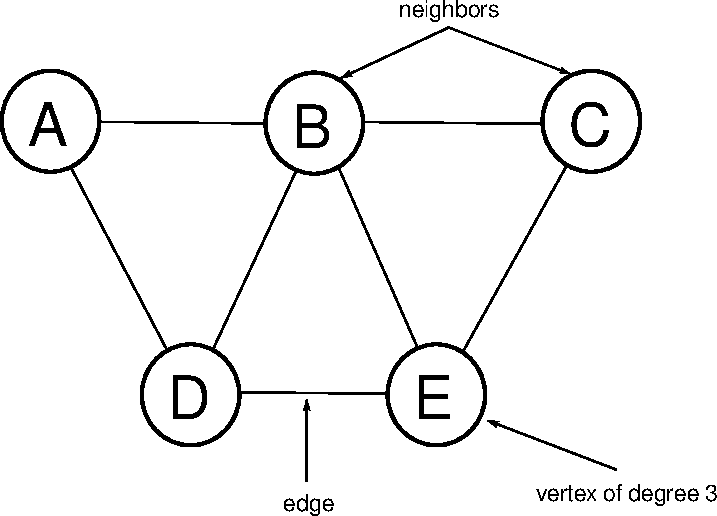
\includegraphics[scale=0.4]{figures/graph.pdf}}
\end{center}
\end{frame}

\begin{frame}[fragile]
\pause

A data type \lstinline{Graph} that represents a graph
\begin{center}
\begin{tabular}{cc}
method & description \\ \hline
\lstinline$Graph(filename, delimiter)$ & \makecell{a new graph $g$ from $filename$ (defaults to \lstinline$None$ representing \\ an empty graph)  using $delimiter$ (defaults to whitespace)} \\
\lstinline$g.addEdge(v, w)$ & add edge $v$-$w$ to $g$ \\
\lstinline$g.adjacentTo(v)$ & an iterable for neighbors of vertex $v$ in $g$ \\
\lstinline$g.vertices()$ & an iterable for vertices in $g$ \\
\lstinline$g.hasVertex(v)$ & is $v$ a vertex in $g$? \\
\lstinline$g.hasEdge(v, w)$ & is $v$-$w$ an edge in $g$? \\
\lstinline$g.countV()$ & number of vertices in $g$ \\
\lstinline$g.countE()$ & number of edges in $g$ \\
\lstinline$g.degree(v)$ & number of neighbors of $v$ in $g$ \\
\lstinline$str(g)$ & string representation of $g$
\end{tabular} 
\end{center}
\end{frame}

\begin{frame}[fragile]
\pause

\begin{framed}
\tiny \lstinline{graph.py}: Definition of \lstinline{Graph} data type.
\end{framed}

\begin{lstlisting}[language=python,style=focusin]
import stdio
import sys
from instream import InStream

class Graph:
    def __init__(self, filename = None, delimiter = None):
        self._e = 0
        self._adj = dict()
        if filename is not None:
            instream = InStream(filename)
            while instream.hasNextLine():
                line = instream.readLine()
                names = line.split(delimiter)
                for i in range(1, len(names)):
                    self.addEdge(names[0], names[i])
                
    def addEdge(self, v, w):
        if not self.hasVertex(v): self._adj[v] = set()
        if not self.hasVertex(w): self._adj[w] = set()
        if not self.hasEdge(v, w):
            self._e += 1
            self._adj[v].add(w)
            self._adj[w].add(v)
            
    def adjacentTo(self, v):
        return iter(self._adj[v])
    
    def vertices(self):
        return iter(self._adj)
\end{lstlisting}
\end{frame}

\begin{frame}[fragile]
\pause

\begin{lstlisting}[language=python,style=focusin]
    def hasVertex(self, v):
        return v in self._adj

    def hasEdge(self, v, w):
        return w in self._adj[v]
    
    def countV(self):
        return len(self._adj)
    
    def countE(self):
        return self._e
    
    def degree(self, v):
        return len(self._adj[v])

    def __str__(self):
        s = ''
        for v in self.vertices():
            s += v + '  '
            for w in self.adjacentTo(v):
                s += w + ' '
            s += '\n'
        return s

def main():
    file = sys.argv[1]
    graph = Graph(file)
    stdio.writeln(graph)

if __name__ == '__main__':
    main()
\end{lstlisting}
\end{frame}

\begin{frame}[fragile]
\pause

\begin{lstlisting}[language={},style=focusin]
$ more tinygraph.txt
A B
A C
C G
A G
H A
B C
B H
\end{lstlisting}

\pause

\begin{lstlisting}[language={},style=focusin]
$ python3 graph.py tinygraph.txt 
A  H C B G 
H  A B 
C  A B G 
B  A H C 
G  A C 

\end{lstlisting}
\end{frame}

\begin{frame}[fragile]
\pause

\begin{framed}
\tiny invert.py: Accept strings $filename$ and $delimiter$ as command-line arguments, build a graph from $filename$, repeatedly read a vertex name from standard input and write the neighbors of that vertex to standard output.
\end{framed}

\begin{lstlisting}[language=python,style=focusin]
import stdio
import sys
from graph import Graph

filename = sys.argv[1]
delimiter = sys.argv[2]
graph = Graph(filename, delimiter)
while stdio.hasNextLine():
    v = stdio.readLine()
    if graph.hasVertex(v):
        for w in graph.adjacentTo(v):
            stdio.writeln('  ' + w)
\end{lstlisting}

\pause

\begin{lstlisting}[language={},style=focusin]
$ python3 invert.py tinygraph.txt " "
C
  A
  B
  G
A
  H
  C
  B
  G
<ctrl-d>
\end{lstlisting}
\end{frame}

\begin{frame}[fragile]
\pause

\begin{lstlisting}[language={},style=focusin]
$ python3 invert.py movies.txt "/"
Bacon, Kevin
  Wild Things (1998)
  My Dog Skip (2000)
  Flatliners (1990)
  Sleepers (1996)
  In the Cut (2003)
  Mystic River (2003)
  JFK (1991)
  She's Having a Baby (1988)
  Few Good Men, A (1992)
  River Wild, The (1994)
  Novocaine (2001)
  Beauty Shop (2005)
  Woodsman, The (2004)
  Tremors (1990)
  Hollow Man (2000)
  Diner (1982)
  Planes, Trains & Automobiles (1987)
  Footloose (1984)
  Where the Truth Lies (2005)
  Murder in the First (1995)
  Animal House (1978)
  Stir of Echoes (1999)
  Trapped (2002)
  Apollo 13 (1995)
  Friday the 13th (1980)
  He Said, She Said (1991)
  Picture Perfect (1997)
<ctrl-d>
\end{lstlisting}
\end{frame}

\section{Shortest Paths in Graphs}
\begin{frame}[fragile]
\pause

Given two vertices in a graph, a path is a sequence of vertices connected by edges, and a shortest path is one with the minimal number of edges over all such paths

\pause
\bigskip

A data type \lstinline{PathFinder} for finding paths in a graph
\begin{center}
\begin{tabular}{cc}
method & description \\ \hline
\lstinline$PathFinder(graph, s)$ & a path finder $pf$ to find all shortest paths from $s$ in $graph$ \\
\lstinline$pf.distanceTo(v)$ & distance between $s$ and $v$ \\
\lstinline$pf.hasPathTo(v)$ & is there a path between $s$ and $v$? \\
\lstinline$pf.pathTo(v)$ & an iterable for the path from $s$ to $v$
\end{tabular} 
\end{center}
\end{frame}

\begin{frame}[fragile]
\pause

\begin{framed}
\tiny pathfinder.py: Definition of \lstinline{PathFinder} data type.
\end{framed}

\begin{lstlisting}[language=python,style=focusin]
import stdio
from queue import Queue

class PathFinder:
    def __init__(self, graph, s):
        self._distTo = dict()
        self._edgeTo = dict()
        queue = Queue()
        queue.enqueue(s)
        self._distTo[s] = 0
        self._edgeTo[s] = None
        while not queue.isEmpty():
            v = queue.dequeue()
            for w in graph.adjacentTo(v):
                if w not in self._distTo:
                    queue.enqueue(w)
                    self._distTo[w] = 1 + self._distTo[v]
                    self._edgeTo[w] = v
    
    def distanceTo(self, v):
        return self._distTo[v]
        
    def hasPathTo(self, v):
        return v in self._distTo

    def pathTo(self, v):
        path = []
        while v is not None:
            path += [v]
            v = self._edgeTo[v]
        return reversed(path)
\end{lstlisting}
\end{frame}

\begin{frame}[fragile]
\pause

\begin{framed}
\tiny separation.py: Accept $filename$, $delimiter$, and a source vertex $s$ as command-line arguments, build a graph from the file, assuming that each line of the file specified a vertex and a list of vertices connected to that vertex, separated by the delimiter, and then repeatedly read a destination vertex from standard input, and write the shortest path from the source to the destination.
\end{framed}

\begin{lstlisting}[language=python,style=focusin]
import stdio
import sys
from graph import Graph
from pathfinder import PathFinder

def main():
    filename = sys.argv[1]
    delimiter = sys.argv[2]
    s = sys.argv[3]
    graph = Graph(filename, delimiter)
    pf = PathFinder(graph, s)
    while stdio.hasNextLine():
        t = stdio.readLine()
        if pf.hasPathTo(t):
            distance = pf.distanceTo(t)
            for v in pf.pathTo(t):
                stdio.writeln('   ' + v)
            stdio.writeln('distance: ' + str(distance))

if __name__ == '__main__':
    main()
\end{lstlisting}
\end{frame}

\begin{frame}[fragile]
\pause

\begin{lstlisting}[language={},style=focusin]
$ python3 separation.py routes.txt " " JFK
LAX   
   JFK
   ORD
   PHX
   LAX
distance: 3
DFW
   JFK
   ORD
   DFW
distance: 2
<ctrl-d>
\end{lstlisting}

\pause

\begin{lstlisting}[language={},style=focusin]
$ python3 separation.py movies.txt "/" "Bacon, Kevin"
Kidman, Nicole
   Bacon, Kevin
   Wild Things (1998)
   Dillon, Matt (I)
   To Die For (1995)
   Kidman, Nicole
distance: 4
Hanks, Tom
   Bacon, Kevin
   Apollo 13 (1995)
   Hanks, Tom
distance: 2
<ctrl-d>
\end{lstlisting}
\end{frame}

\section{Small-World Graphs}
\begin{frame}[fragile]
\pause

Small-world graphs are characterized by the following three properties

\begin{enumerate}
\item They are sparse: the number of vertices is much smaller than the number of edges

\item They have short average path lengths: if you pick two random vertices, the length of the shortest path between them is short

\item They exhibit local clustering: if two vertices are neighbors of a third vertex, then the two vertices are likely to be neighbors of each other
\end{enumerate}
\end{frame}

\begin{frame}[fragile]
\pause

\begin{framed}
\tiny smallworld.py: A module for computing the small-world properties of a graph.
\end{framed}

\begin{lstlisting}[language=python,style=focusin]
import instream
import stdio
import sys
from graph import Graph
from pathfinder import PathFinder

def averageDegree(graph):
    return 2.0 * graph.countE() / graph.countV()

def averagePathLength(graph):
    total = 0
    for v in graph.vertices():
        pf = PathFinder(graph, v)
        for w in graph.vertices():
            total += pf.distanceTo(w)
    return 1.0 * total / (graph.countV() * (graph.countV() - 1))

def clusteringCoefficient(graph):
    total = 0
    for v in graph.vertices():
        possible = graph.degree(v) * (graph.degree(v) - 1)
        actual = 0
        for u in graph.adjacentTo(v):
            for w in graph.adjacentTo(v):
                if graph.hasEdge(u, w):
                    actual += 1
        if possible > 0:
            total += 1.0 * actual / possible
    return total / graph.countV()
\end{lstlisting}
\end{frame}

\begin{frame}[fragile]
\pause

\begin{lstlisting}[language=python,style=focusin]
def main():
    graphFile = sys.argv[1]
    delimiter = sys.argv[2]
    graph = Graph(graphFile, delimiter)
    vertexCount = graph.countV()
    edgeCount = graph.countE()
    stdio.writef('%d vertices, %d edges\n', vertexCount, edgeCount)
    avgDegree = averageDegree(graph)
    stdio.writef('average degree         = %7.3f\n', avgDegree)
    avgPathLength = averagePathLength(graph)
    stdio.writef('average degree         = %7.3f\n', avgPathLength)
    clusteringCoef = clusteringCoefficient(graph)
    stdio.writef('clustering coefficient = %7.3f\n', clusteringCoef)

if __name__ == '__main__':
    main()
\end{lstlisting}

\pause

\begin{lstlisting}[language={},style=focusin]
$ python3 smallworld.py tinygraph.txt " "
5 vertices, 7 edges
average degree         =   2.800
average degree         =   1.300
clustering coefficient =   0.767
\end{lstlisting}
\end{frame}

\begin{frame}[fragile]
\pause

\begin{framed}
\tiny performer.py: Accept $filename$, the name of a movie-cast file and a $delimiter$ as command-line arguments and create the associated performer-performer graph. Then write to standard output the number of vertices, the average degree, the average path length, and the clustering coefficient of the graph.
\end{framed}

\begin{lstlisting}[language=python,style=focusin]
import smallworld
import stdio
import sys
from graph import Graph
from instream import InStream

def main():
    filename  = sys.argv[1]
    delimiter = sys.argv[2]
    graph = Graph()
    instream = InStream(filename)
    while instream.hasNextLine():
        line = instream.readLine()
        names = line.split(delimiter)
        for i in range(1, len(names)):
            for j in range(i+1, len(names)):
                graph.addEdge(names[i], names[j])
    degree  = smallworld.averageDegree(graph)
    length  = smallworld.averagePathLength(graph)
    cluster = smallworld.clusteringCoefficient(graph)
    stdio.writef('number of vertices     = %d\n', graph.countV())
    stdio.writef('average degree         = %7.3f\n', degree)
    stdio.writef('average path length    = %7.3f\n', length)
    stdio.writef('clustering coefficient = %7.3f\n', cluster)

if __name__ == '__main__':
    main()
\end{lstlisting}
\end{frame}

\begin{frame}[fragile]
\pause

\begin{lstlisting}[language={},style=focusin]
$ cat tinymovies.txt
Movie 1/Actor A/Actor B/Actor H
Movie 2/Actor B/Actor C
Movie 3/Actor A/Actor C/Actor G
\end{lstlisting}

\pause

\begin{lstlisting}[language={},style=focusin]
$ python3 performer.py tinymovies.txt "/"
number of vertices     = 5
average degree         =   2.800
average path length    =   1.300
clustering coefficient =   0.767
\end{lstlisting}

\pause

\begin{lstlisting}[language={},style=focusin]
$ python3 performer.py moviesg.txt "/"
number of vertices     = 19044
average degree         = 148.688
average path length    =   3.494
clustering coefficient =   0.911
\end{lstlisting}
\end{frame}
\end{document}
